% Section 3 — Method (Draft)
% OntoCoDec: Type-Valid Information Extraction
% via Compiled Ontology Constraints

\section{Method}
\label{sec:method}

\begin{figure*}[t]
\centering
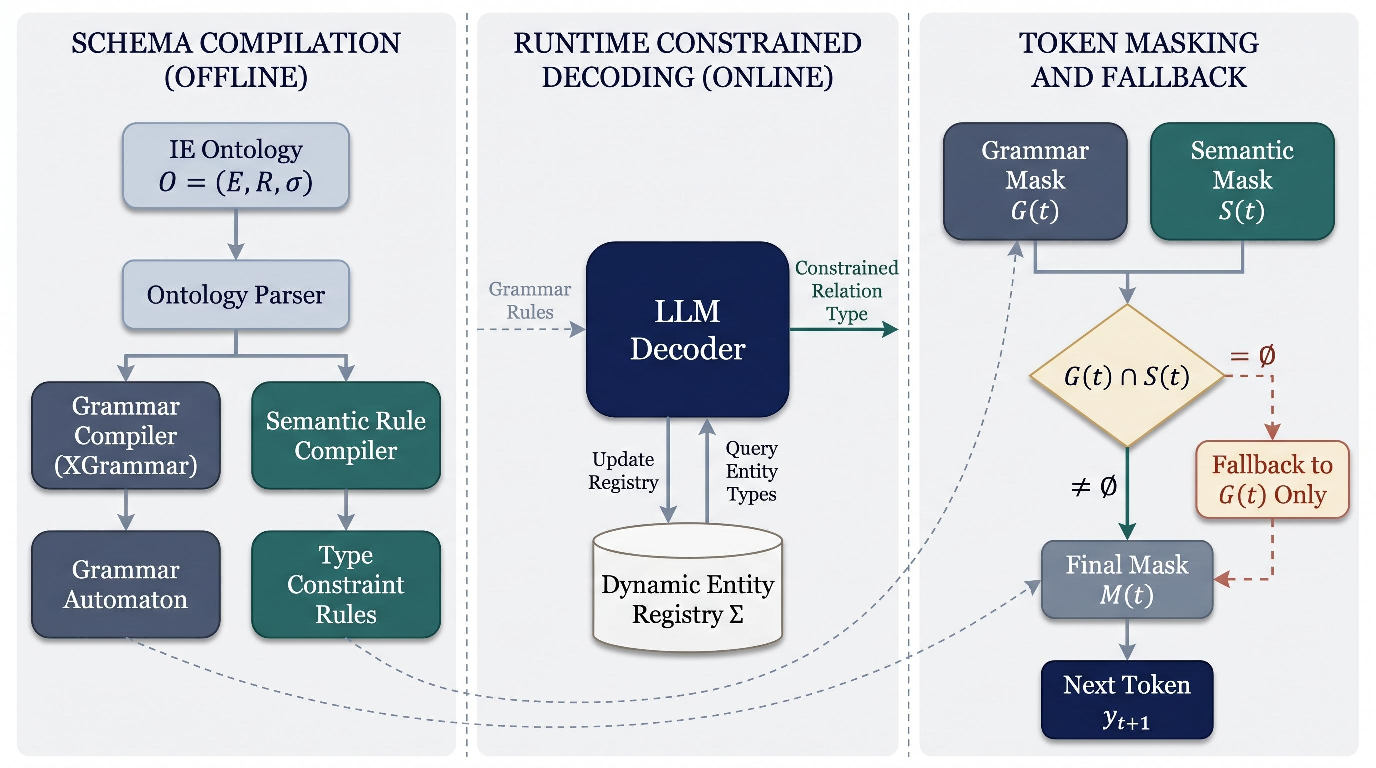
\includegraphics[width=\textwidth,height=6.5cm,keepaspectratio]{figures/fig1_framework.pdf}
\caption{Overview of OntoCoDec. An IE ontology is compiled into two constraint layers: a grammar layer (context-free) and a semantic layer (prefix-decidable with state). At each decoding step, the final mask $M_{\text{final}}(t) = G(t) \cap S(t)$ ensures both structural and type validity; when $S(t) \cap G(t) = \emptyset$, grammar-first fallback preserves JSON integrity.}
\label{fig:framework}
\end{figure*}


\paragraph{Preliminaries.}
\label{sec:preliminaries}
An IE ontology $\mathcal{O} = (\mathcal{E}, \mathcal{R}, \sigma)$ defines entity types $\mathcal{E}$, relation types $\mathcal{R}$, and a mapping $\sigma: \mathcal{R} \to \mathcal{P}(\mathcal{E} \times \mathcal{E})$ specifying valid (head type, tail type) pairs per relation.
A triple $(h, r, t)$ is \emph{type-valid} if $(\mathrm{type}(h), \mathrm{type}(t)) \in \sigma(r)$.
We quantify constraint restrictiveness via \emph{constraint tightness} $\kappa(r)$ (\S\ref{sec:composition}); empirical constraints achieve 99\%+ instance-level coverage (SciERC 99.0\%, DocRED 99.4\%), with grammar-first fallback (\S\ref{sec:composition}) ensuring no valid triples are blocked.
Given $\mathcal{O}$ and an autoregressive LM $\mathcal{M}$, we seek constraints $\mathcal{C}$ ensuring: (a)~\textbf{structural validity}, i.e., well-formed JSON with $\mathcal{E}$/$\mathcal{R}$ membership; and (b)~\textbf{type validity}, i.e., $(\mathrm{type}(h), \mathrm{type}(t)) \in \sigma(r)$ for every triple.
Condition (a) is context-free; (b) is context-sensitive but \emph{prefix-decidable}: at the point where a type token is generated, all information needed is available in the decoded prefix.

\smallskip
\noindent
We present OntoCoDec, a framework that translates IE ontologies into token-level constraints enforced during autoregressive generation.
The design is guided by a decidability analysis of IE type constraints.

\paragraph{Constraint decidability taxonomy.}
\label{sec:decidability}
We classify IE type constraints into three levels: (1)~\emph{context-free}: vocabulary membership and JSON structure; (2)~\emph{prefix-decidable with state}: domain/range type validity, determined at each type-bearing position given the decoded relation type and entity registry; (3)~\emph{non-local}: cross-entity type consistency, which depends on the full output.
Unlike code generation where types are statically declared, IE constraints fall into level~2: entity types are inferred from text, the registry is built dynamically, and constraint targets depend on the co-occurring relation.
OntoCoDec enforces levels 1--2 (grammar and semantic layers, respectively); level~3 is addressed by beam search or post-hoc resolution (Appendix~\ref{app:tcr}).

\smallskip
\noindent
Existing grammar-constrained decoding frameworks (e.g., XGrammar) enforce level~1 constraints (structural validity and vocabulary membership) but IE domain/range rules require cross-position entity-type state that context-free grammars cannot express.
Even when the entity set is finite, encoding type constraints into a deterministic finite automaton (DFA) requires $O(|\mathcal{E}|^{|\text{entities}|})$ states: for typical SciERC documents (median 17 entities, 6 types), $6^{17} \approx 1.6{\times}10^{13}$ states; for DocRED (median 19 entities, 6 types), $6^{19} \approx 6.1{\times}10^{14}$, well beyond practical construction for online decoding.
While cross-reference binding is known to exceed context-free expressiveness in programming language theory, its implications for IE-specific type constraints (where entity types are inferred from text rather than statically declared) have not been formally characterized.
Formally, domain/range constraints for unbounded entity sets are not context-free (\textbf{Proposition~1}; proof via pumping argument in Appendix~\ref{app:pumping-lemma}): a pushdown automaton (PDA) cannot retrieve the type of entity $e_k$ without destroying stack entries above it.
OntoCoDec's semantic layer addresses this with a runtime entity registry $\mathcal{D}$ (a finite map enabling random-access type lookups), avoiding both the theoretical impossibility (unbounded) and the engineering intractability (finite but exponential).

\noindent\textbf{Empirical Observation} (scale-dependent enabling dependency)\textbf{.} The grammar layer alone cannot enforce domain/range constraints (Proposition~1), while the semantic layer alone achieves only 24\% DR reduction at 8B without grammar-enforced vocabulary membership (\S\ref{sec:scierc-results}, Table~\ref{tab:scierc-ablation}).
The strength of this dependency is scale-dependent: at 70B, the semantic layer independently achieves 84\% DR reduction (\S\ref{sec:70b-results}), whereas 8B models show only 24\% independent reduction.
\smallskip

We describe the problem formulation (\S\ref{sec:formulation}), each layer, and two decoding strategies (\S\ref{sec:strategies}); formal analysis of constraint composition is in Section~\ref{sec:composition}.


\subsection{Problem Formulation}
\label{sec:formulation}

\paragraph{IE as structured generation.}
Given an input text $x$, a language model generates a structured JSON output $y$:
%
\begin{equation}\label{eq:output-schema}
\resizebox{.88\columnwidth}{!}{$\displaystyle
  y = \bigl\{\texttt{entities}: [\{n_i, \tau_i\}],\; \texttt{relations}: [\{h_j, t_j, r_j, \tau^h_j, \tau^t_j\}]\bigr\}
$}
\end{equation}
%
where each entity has a name $n_i$ and type $\tau_i \in \mathcal{E}$, and each relation specifies head $h_j$, tail $t_j$, relation type $r_j \in \mathcal{R}$, and head/tail entity types $\tau^h_j, \tau^t_j$.
The output JSON Schema (\S\ref{sec:grammar}) enforces a fixed field ordering (head $\to$ tail $\to$ relation $\to$ head\_type $\to$ tail\_type) via deterministic grammar compilation, ensuring the relation type $r_j$ is known before entity type fields and enabling sequential domain/range lookups (\S\ref{sec:dynamic-masking}).
The grammar structurally enforces entity-before-relation ordering (maintained in all documents across all configurations), ensuring the entity registry (\S\ref{sec:entity-registry}) is populated before relation-level type constraints are evaluated; unregistered entities trigger domain-only filtering.

\paragraph{Ontology compliance.}
Using the ontology $\mathcal{O} = (\mathcal{E}, \mathcal{R}, \sigma)$ defined above, we write $\operatorname{dom}(r) = \{\tau^h : \exists \tau^t,\, (\tau^h, \tau^t) \in \sigma(r)\}$ for domain-valid head types and $\operatorname{range}(r, \tau^h) = \{\tau^t : (\tau^h, \tau^t) \in \sigma(r)\}$ for the conditional range given head type $\tau^h$.
Our enforcement target is \emph{pair-based} type validity: $(\tau^h, \tau^t) \in \sigma(r)$ for every triple.
The decoder enforces this sequentially: $\tau^h \in \operatorname{dom}(r)$ at head position, then $\tau^t \in \operatorname{range}(r, \tau^h)$ at tail position, achieving best-effort pair-based enforcement (pair validity ensured when no fallback is triggered; domain-only filtering otherwise) strictly stronger than independent domain/range checks (which over-permit 33--37\% spurious pairs on SciERC/DocRED; \S\ref{sec:rectangularity}).


\subsection{Grammar Layer}
\label{sec:grammar}

A JSON Schema encoding Eq.~\eqref{eq:output-schema} with \texttt{enum} constraints ($\mathcal{E}$, $\mathcal{R}$) is compiled into a pushdown automaton via XGrammar~\cite{dong2025xgrammar}.
At step $t$, grammar-valid tokens $G(t) \subseteq V$ pass; all others receive logits $-\infty$, enforcing structural validity, vocabulary membership ($r_j \in \mathcal{R}$, $\tau_i \in \mathcal{E}$), but not domain/range constraints (which depend on entity types within each triple).

\subsection{Semantic Layer}
\label{sec:semantic}

The semantic layer enforces domain/range constraints through a stateful logits processor maintaining an entity registry during generation.
\emph{Running example}: for \textsc{Used-for} ($\operatorname{dom}{=}\{\textrm{Method}\}$, $\operatorname{range}{=}\{\textrm{Task}\}$), entity ``ResNet'' (Method) passes the head-type check while Material is blocked; ``image classification'' (Task) passes the tail-type check.

\paragraph{Entity registry.}
\label{sec:entity-registry}
The semantic layer builds a registry $\mathcal{D}: \text{name} \to \text{type}$ incrementally during entity generation: each completed entry $\{n_i, \tau_i\}$ adds $(n_i, \tau_i)$ to $\mathcal{D}$, which is consulted during relation generation for type lookups.
The registry uses \emph{first-seen} semantics: when an entity name appears in multiple triples, the type assigned at its first occurrence governs all subsequent constraint checks, making type enforcement sensitive to generation order.
At each step $t$, the processor pattern-matches the decoded prefix to identify the current field position; semantic masks activate only at type-bearing positions (\textsc{HeadType}, \textsc{TailType}).
\label{sec:position-detection}

\paragraph{Dynamic masking.}
\label{sec:dynamic-masking}
At type-bearing positions, the processor computes a semantic mask $S(t) \subseteq V$.
At a \textsc{HeadType} position, if $h_j \in \mathcal{D}$ and $\mathcal{D}[h_j] \in \operatorname{dom}(r_j)$, the mask allows only the registered type; otherwise it falls back to all domain-valid types $\operatorname{dom}(r_j)$.
At a \textsc{TailType} position, the mask restricts to $\operatorname{range}(r_j, \tau^h_j)$ conditioned on the already-determined head type, further narrowing to the registered type when $t_j \in \mathcal{D}$.
This sequential check achieves best-effort pair-based enforcement (\S\ref{sec:formulation}), strictly tighter than independent domain/range checking; ``best-effort'' reflects the grammar-first fallback (\S\ref{sec:composition}), which prioritizes JSON integrity over type validity when constraints conflict.

\paragraph{Tokenizer-agnostic type masking.}
We use \emph{continuation masking} to handle context-dependent tokenizations and prefix-shared types (e.g., \textsc{Sen}/\textsc{Sid}/\textsc{Side} in WikiEvents): a compile-time prefix map identifies valid continuations for each type name, disambiguating over multiple steps across byte-level byte pair encoding (BPE) (Qwen, Llama) and SentencePiece (Mistral).

\paragraph{Grammar-semantic interaction.}
\label{sec:interaction}
The final mask is $G(t) \cap S(t)$; when empty, grammar-first fallback applies (\S\ref{sec:composition}), embodying this interaction: semantic constraints reduce DR by only 24\% without grammar-enforced vocabulary.


\subsection{Decoding Strategies}
\label{sec:strategies}

\paragraph{S1 (joint extraction): Single-pass decoding.}
Both layers are active throughout generation; the entity registry populates during entity decoding and is immediately available for relation-level type checking.

\paragraph{S2 (two-pass pipeline): Two-pass decoding.}\label{sec:s2}
A first pass extracts entities; these compile an input-dependent grammar for the second pass.
S1 achieves higher R-F1 at comparable DR (\S\ref{sec:scierc-results}) and is the primary configuration.
